\subsubsection{Opportunities}\label{subsub:4_opportunities}


\paragraph{\textbf{API http-code response}}\label{swot:o_api_http_responsecode}:
The return actions from the called APIs are not provided with a code but text.
As proof of concept, calls were made from Postman~(see figure~\ref{fig:postman-get-person}) to Ampersand and that worked as expected.
(Ref. to \nameref{s:1_8_api})
\begin{figure}[ht]
    \centering
    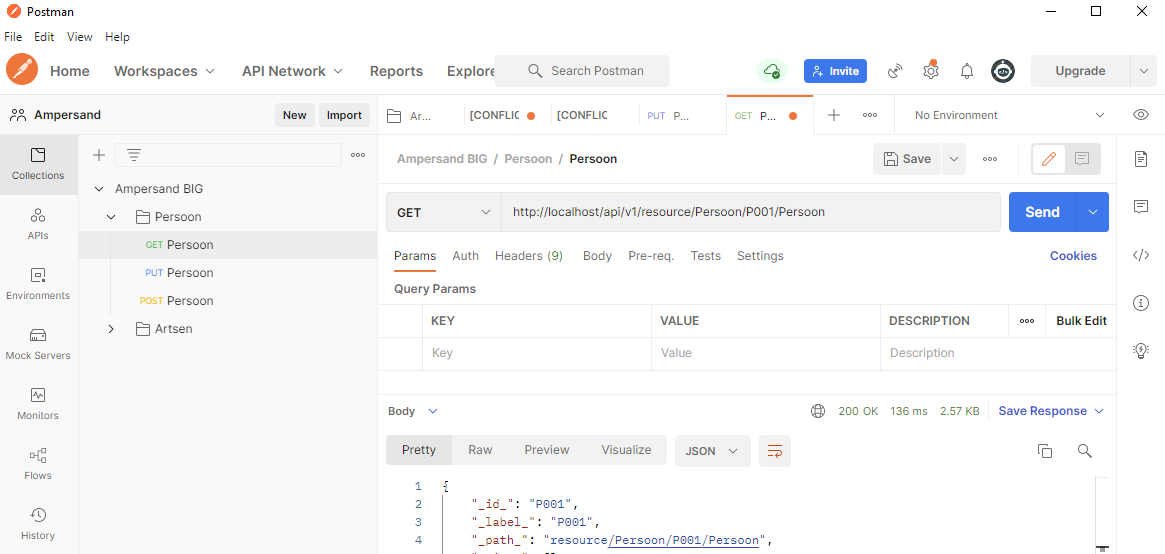
\includegraphics[width=\textwidth]{/postman_GET.PNG}
    \caption{Postman GET Person}
    \label{fig:postman-get-person}
\end{figure}

\paragraph{\textbf{Customization \acrshort{rk}}}\label{swot:o_customization}:
An organized ICT organization such as the \acrshort{cibg} has an architecture that new software must comply with.
One of the developments in the \acrshort{cibg} is the set-up of the \acrshort{rk} (see interview developer Appendix~\ref{par:interview-developer}).
\acrlong{rk} its terminology includes "zaken" and "producten".
Every service, read implementation of a law, we call a product.
There are default items that always appear in every registry.
These are pre-modeled in \acrshort{rk}.
This includes a foundation for each registry and can be expanded to meet the needs of the registry.
The basis is the minimum common denominator of the registers, extendable to specific elements arising from the law.
There is certainly overlap in the data obtained from the analysis of the great law and the \acrshort{rk}.
About 80\% of the \acrshort{rk} is generic and the other 20\% is custom.
All new registers therefore have the same basic principles and largely run on the same software.
However, a mapping still has to take place from the found Concepts from the law to \acrshort{rk}.
The overlap in this is not always immediately visible.
Within the \acrshort{rk} the term product is used, within the \acrshort{big} this product is a register or possibly even all registers.
The latter depends on the implementation.
This mapping must be made explicit and has not been taken into account in this study.
The developer has indicated that full integration of the Ampersand model is not possible, due to the aforementioned overlap of the Concepts.
However, the modified part of the \acrshort{rk} can be used for the Ampersand model implementation.
Although Ampersand is new to the \acrshort{cibg} organization, one of the interviewees pointed out (see interview analist~\ref{par:interview-analist}) that documentation in the form of a design should be made with each new register.
According to the analyst, it should not matter which tool is used for this.
The advantage of Ampersand is that it generates a model from the analysis instead of the usual model-to-text approach.
A model is made of each pattern.
See for example the Pattern for \mbox{Person} (see script~\ref{lst:persoon}).
This results in the model of figure~\ref{fig:pattern-persoon}.
\begin{figure}[H]
    \centering
        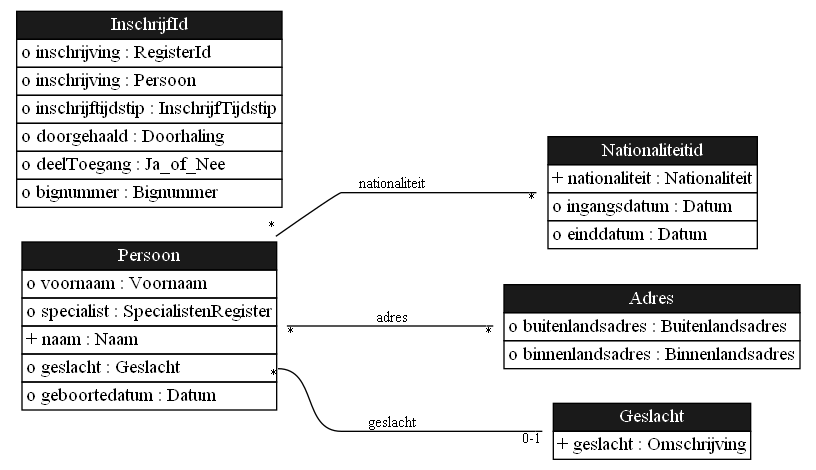
\includegraphics[width=1\textwidth]
            {../images/CDPatternPersoon.png}
        \caption{Pattern Persoon}
    \label{fig:pattern-persoon}
\end{figure}
Calculations are not standard in Ampersand, but this can be solved by writing external functions or even solving it in \acrshort{rk}.
(Ref. to  \nameref{s:5_2_demarcation}, \nameref{s:1_7_architecture_and_registerkern}, \nameref{s:4_1_architectural_fit}, \nameref{s:1_10_ampersand_design_method}, \nameref{s:2_7_organisation_ampersand_use}, \nameref{s:4_7_total_design})

\paragraph{\textbf{Version-gap analysis}}\label{swot:o_version_gap_analysis}:
Although it is not the intention to use Ampersand prototype in a production environment, it is useful to save the data entered in an earlier version and use it in later versions.
In ``\nameref{swot:w_data_migration}'' included with the weaknesses we indicate that this is a problem and it would be a good addition to develop a tool in Ampersand that focuses on preserving data across versions.
(Ref. to \nameref{s:3_5_model_maintenance})

\paragraph{\textbf{Atlas local}}\label{swot:o_atlas_local}:
In RAP there is a tool called Atlas, it shows the context and the patterns.
In addition, all Concepts, Rules, Properties and Relations, with hyperlinks to the components.
Via the hyperlink details of the item inclusion a relationship diagram is shown, very nicely executed and very useful when working in RAP.
This tool is a viewer on the information and it is not possible to also edit the \F{information in Atlas}{Being able to edit the Atlas information from Atlas}.
However, the case study was so large that the RAP environment was not sufficient.
RAP does not support Includes and has been used extensively.
Unfortunately, \F{Atlas availability}{Make Atlas available outside the RAP environment.} cannot be implemented outside of RAP.

As a novice user of Ampersand it takes a while to master Relation algebra.
That is why an excel sheet has been made to make the Relations visible with the associated multiplicity.
This is a method that is easy to use initially.
The disadvantage of this approach is the consistent transfer of Concepts and Relations.
We need to double track this information and redundancy in the field of data will certainly go wrong.
When Concepts disappear, they must also be removed from Excel or Relations that do change due to new insights must be adjusted here.
In short, this does work for small, well-arranged projects, but for larger ones, gaps will quickly arise and this no longer represents reality.
The result was that the excel sheet was used a lot in the beginning and not anymore later on.
(Ref. to \nameref{s:3_5_model_maintenance}, \nameref{s:2_2_multiplicity})

\paragraph{\textbf{\acrlong{ca} as testbasis}}\label{swot:o_ca_as_testbasis}:
By using Ampersand as a design tool, a prototype is available at an early stage.
This prototype can be converted into a website with the appearance of a \acrshort{cibg} website by means of HTML additions and CSS adjustments.
Test cases can already be developed at an early stage on the basis of this prototype and the functions of the prototype, by using the APIs, can be used as a stub in the development of the system.
(Ref. to \nameref{s:2_6_prototype_use}, \nameref{s:1_10_ampersand_design_method})

\paragraph{\textbf{Stub}}\label{swot:o_stub}:
The prototype can be accessed through APIs.
In principle it is possible to use the prototype in whole or in part as a stub.
When developing the application, based on the \acrshort{ca}, the prototype can be used in the form of a stub.
(Ref. to \nameref{s:4_5_test_scenario})


\paragraph{\textbf{Annotation}}\label{swot:o_annotation}:
To maintain an overview when performing the textual analysis, it is necessary to use a annotation (see section~\ref{subsection:ampersand-knowledge}, heading~\nameref{subsub:1_annotation}).
Annotation would be a nice addition to Ampersand.
It does introduce a close link between Ampersand and the source document.
(Ref. to \nameref{s:1_3_source_handling})